
\subsection{Informacion y Entropia}

Siguiendo con lo dicho en la introducción podemos identificar de acuerdo a lo
publicado en \textit{A Mathematical Theory of Communication} (Ver \cite{shannon}) ciertos elementos
comunes a toda comunicación. Pricipalmente contaremos con un \textit{Emisor} el
cual transmite una \textit{Fuente de información} por medio de un canal
asediado por una \textit{Fuente de ruido} que impacta durante su trayecto a la
señal mas tarde recibida por un \textit{Receptor}. De acuerdo a Claude E.
Shannon, si conocemos el proceso aleatorio que genera el ruido, es posible
recuperar la información transmitida asumiendo que dicha perturbación se
comporta como un proceso gaussiano con una varianza conocida, usualmente al que
se asocia a la noción de ruido blanco. A este esquema se lo puede expresar
ilustrativamente de la siguiente forma:

\begin{figure}[ht]
\begin{center}
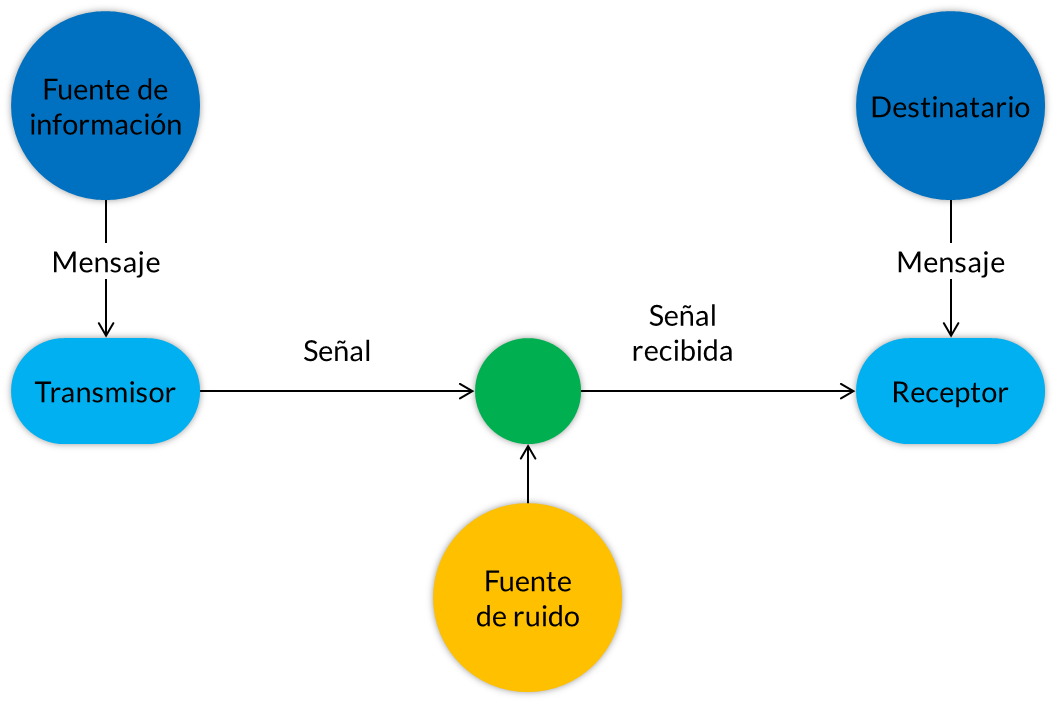
\includegraphics[width=0.6\columnwidth]{EsquemaShannon.png}
\caption{Diagrama de comunicación}
\end{center}
\end{figure}


A la hora de entablar una comunicación es necesario que las partes involucradas
se pongan de acuerdo sobre un lenguaje en común con el que van a desarrollar el
\quotes{dialogo} a lo largo del tiempo. Para poder llevar esto a cabo es que se
necesita definir un conjunto de símbolos $S = \{ s_1, ..., s_n \}$ que aporten
semantica a lo que se tratando de transmitir. De acuerdo al análisis de Shannon
cada uno de estos símbolos tiene asociada una cantidad de información que
responde a la formula $I(s_i) = log(\frac{1}{p(s_i)})$, donde $I(s_i)$ es la
información asociada a $s_i$ para cada $i$ con $1 \leq i \leq n$. Algo
importante a notar para entender esta formula es que la información de un
símbolo estará íntimamente relacionada con su probabilidad, a modo
coloquial, podemos pensar que en cuanto mas probable sea un símbolo, mas
esperable será su aparición, y por lo tanto mas predecible. En constraste
aquellas apariciones de símbolos poco probables son considerados un evento
desentonante con respecto a mucho mas usuales, por lo que se les da mas valor
semántico. En base a ello podemos observar que dicha definición cumple con
ciertas condiciones naturales para el calculo de de la información:

\begin{itemize}
	\item Si $p(s_i) = 1$ para algun $i$, entonces $I(s_i) = 0$, ya que un evento que ocurre siempre no aporta información significativa
	\item Si $s \in S$, entonces $I(s) \geq 0$. Esto vale ya que la inversa de la probabilidad es siempre mayor o igual a 1
\end{itemize}

\subsection{Entropía}

Ademas nos interesará otra noción importante, la de \textit{Entropía}. 
Esta refleja el promedio de la información
obtenida de una fuente en base a las probabilidad de ocurrencia e información
que provee cada símbolo en la comunicación, o, de otra manera, el nivel de
desorden de la comunicación.  

\begin{definicion} \label{eq:entropia}
Sea $S$ una fuente de información. Se define $H(S)$ la entropía de la fuente como a continuación.

\begin{equation} 
	H(S) = \sum\limits_{i=1}^n p(s_i)I(s_i)
\end{equation}

\end{definicion}

Por ejemplo, al ser todos los símbolos, igualmente probables,
la entropía será máxima alcanzando el valor de $log_2(\lvert simbolos\rvert)$.
De esta ultima observación se desprende, de forma general, que cuanto mayor sea el grado de
\quotes{equiprobabilidad} de los símbolos de la fuente, mayor será la
\textit{Entropía}, no superando al máximo posible (en el caso equiprobable).
Por el contrario sera mucho menor para aquellas fuentes en las
que la distribución de probabilidades sea muy desigual (siempre por encima de cero).
Esto será de vital importancia para los análisis posteriores.
\\

La longitud promedio de un código es $L(C) = \sum_{s \in S} P(s)l(C(s))$ donde
$l(C(s))$ es la largo de la codificación de S.
\\

\subsection{Compresibilidad}

Otra noción que se introduce en este trabajo es la de \textit{Compresibilidad}
\begin{definicion}
Sea $S$ una fuente de información, definimos el nivel de \textit{Compresibilidad} de S como
\begin{equation} \label{eq:eta_c}
	\eta_{C}(S)=\frac{H_{max}(S) - H(S)}{H_{max}(S)}
	\end{equation}donde $H(S)$ es la entropía de la
	fuente (ver Definición \ref{eq:entropia}) y $H_{max}(S)$ la entropía máxima.
\end{definicion}

Cuando $H(S) = H_{max}(S)$ decimos que
la fuente no es muy compresible debido a que la única forma optima e instantánea
de codificar los símbolos es que todos tengan la misma longitud. Por otro lado
si $H(S) << H_{max}(S)$ \footnote{Entiéndase $A << B$ como $A$ mucho menor que $B$} y asignamos a símbolos más frecuentes
una longitud mas chica que al resto. Permitiendo esto que la longitud promedio
sea menor y por tanto, la longitud promedio de los códigos que se transmitan
mucho mas bajos.
Es por eso que esta formula intenta representar el grado de compresión de la fuente.
Cuanto mas cercano este coeficiente es a cero o uno sera posible comprimir menos
o mas la fuente respectivamente.

\subsection{Protocolo ARP}
Durante los experimentos se analizaron los paquetes ARP. Estos tipo de paquetes
son de control interno de la red que permiten comunicar, mediante distintos mensajes,
que dirección \textbf{IP} le corresponde a qué dirección \textbf{MAC}. Cada dispositivo
cuenta con una caché de estas traducciones para poder efectivamente
transmitir paquetes \textbf{IP} (Capa 3, en el modelo \textbf{OSI}) por la red embebidos
en paquetes \textbf{MAC} (Capa 2, en el modelo \textbf{OSI}). Para esto existen
dos tipos de operaciones, \textit{who-has} e \textit{is-at}. Cuando un nodo A
de la red desea conocer cual es dispositivo B que tiene cierta \textbf{IP} (ie. 192.168.0.1)
éste transmite un mensaje \textit{broadcast} \textit{who-has} con el campo \emph{Target Protocol Address}:192.168.0.1.
Al dispositivo B, con esta IP, le llega este mensaje (eventualmente le llega a todos pero solo B responde ya que es el único con esta IP)
responde con el tipo de operación \textit{is-at} unicast a A (puede debido a que en el paquete está la dirección de source
que es la \textbf{MAC} address del dispositivo A). A A, le llega esta respuesta y con eso agrega a las traducciones esta IP con la respectiva mac adress
recibida. Las entradas de la caché cuentan con un tiempo de expiración debido a posibles cambios de IP de los dispositivos. Finalmente
es por esto último que pasado el tiempo de expiración se vuelve a realizar este protocolo \footnote{Este protocolo se describe en el RFC 826, ver en \url{https://tools.ietf.org/html/rfc826}}

\subsection{Paquetes de red}

En las redes de comunicación informáticas, la información se mueve a través de
ellas en forma de paquetes. Dichos paquetes cuentan con varios campos (se
agregan a medida que los paquetes viajan por el stack \textbf{OSI}, ver \cite[Capítulo 1, p.~32]{compnetworks}), en este
trabajo para modelar las fuentes nos interesaremos en los paquetes de tipo $Ethernet$ \footnote{O en su defecto 802.11 (en las redes Wi-Fi)} e $IP$. En el caso
de $Ethernet$, los campos son:

\begin{enumerate}
	\item MAC orgen
	\item MAC destino
\end{enumerate}

Mientras que en los paquetes ARP de capa 3 nos interesan los campos:

\begin{enumerate}
	\item MAC de origen
	\item IP de origen
	\item MAC de destino
	\item IP de destino
\end{enumerate}
